\documentclass[paper=a4,11pt,parskip=half,toc=listof]{scrartcl}

% % % % % LANGUAGE % % % %
\usepackage{etoolbox} % Allow advanced, programming-like commands like \newtoggle
\newtoggle{german} % Make your choic here
%\togglefalse{german} % English
\toggletrue{german} % German
% % % % % \LANGUAGE % % % %

\usepackage[utf8]{inputenc} % input files werden als utf8 interpretiert
\usepackage[T1]{fontenc} % die schriftart wird mit T1 codiert (will man haben)

\iftoggle{german}{
\usepackage[ngerman]{babel} % Deutsche Sprachanpassungen
\usepackage[german=quotes]{csquotes} % Anfuehrungszeichen
}{
\usepackage[english]{babel} % Deutsche Sprachanpassungen
\usepackage[english=american]{csquotes} % Anfuehrungszeichen
}
\usepackage[resetlabels,labeled]{multibib}
%% The new list's label is "New" and will be titled "The other list".
%% To put cites into this list, use \citeNew.
\newcites{New}{The other list}

\usepackage{scrpage2}
\usepackage{listings}
\usepackage{booktabs}
\usepackage{color}
\usepackage{textcomp}
\usepackage{mathtools}
\usepackage{nicefrac}
\usepackage{amsmath}
\usepackage{cite}
\usepackage{graphicx}
\usepackage{longtable}
\usepackage{float}
\usepackage{setspace}
\usepackage{url}
\usepackage{tabularx}
\usepackage{ltxtable}
\usepackage[table,xcdraw]{xcolor}
\usepackage{colortbl}
\usepackage{hhline}
\usepackage{makecell}
\usepackage{multirow}
\usepackage{wrapfig}
\usepackage{pdfpages}
\usepackage{amssymb}
\usepackage{graphicx}
\usepackage[font=small]{caption} % very thin
\usepackage{subcaption}
\usepackage{picinpar}
\usepackage{fancybox}
\usepackage{pgfkeys}
\usepackage{pifont}
\newcommand{\cmark}{\ding{51}}%
\newcommand{\xmark}{\ding{55}}%
\usepackage[edges]{forest}%dir tree
\definecolor{folderbg}{RGB}{124,166,198}
\definecolor{folderborder}{RGB}{110,144,169} 
\definecolor{folderbg}{RGB}{124,166,198}
\definecolor{folderborder}{RGB}{110,144,169}
\newlength\Size
\setlength\Size{4pt}
\tikzset{%
  folder/.pic={%
    \filldraw [draw=folderborder, top color=folderbg!50, bottom color=folderbg] (-1.05*\Size,0.2\Size+5pt) rectangle ++(.75*\Size,-0.2\Size-5pt);
    \filldraw [draw=folderborder, top color=folderbg!50, bottom color=folderbg] (-1.15*\Size,-\Size) rectangle (1.15*\Size,\Size);
  },
  file/.pic={%
    \filldraw [draw=folderborder, top color=folderbg!5, bottom color=folderbg!10] (-\Size,.4*\Size+5pt) coordinate (a) |- (\Size,-1.2*\Size) coordinate (b) -- ++(0,1.6*\Size) coordinate (c) -- ++(-5pt,5pt) coordinate (d) -- cycle (d) |- (c) ;
  },
}

\forestset{%
  declare autowrapped toks={pic me}{},
  declare boolean register={pic root},
  pic root=0,
  pic dir tree/.style={%
    for tree={%
      folder,
      font=\ttfamily,
      grow'=0,
    },
    before typesetting nodes={%
      for tree={%
        edge label+/.option={pic me},
      },
      if pic root={
        tikz+={
          \pic at ([xshift=\Size].west) {folder};
        },
        align={l}
      }{},
    },
  },
  pic me set/.code n args=2{%
    \forestset{%
      #1/.style={%
        inner xsep= 2\Size,
        pic me={pic {#2}},
      }
    }
  },
  pic me set={directory}{folder},
  pic me set={file}{file},
}

% XML Listing options
\definecolor{dkgreen}{rgb}{0,0.6,0}
\definecolor{mauve}{rgb}{0.58,0,0.82}
\definecolor{gray}{rgb}{0.4,0.4,0.4}
\definecolor{darkblue}{rgb}{0.0,0.0,0.6}
\definecolor{lightblue}{rgb}{0.0,0.0,0.9}
\definecolor{cyan}{rgb}{0.0,0.6,0.6}
\definecolor{darkred}{rgb}{0.6,0.0,0.0}

\lstset{
  basicstyle=\ttfamily\footnotesize,
  columns=fullflexible,
  showstringspaces=false,
  numbers=left,                   % where to put the line-numbers
  numberstyle=\tiny\color{gray},  % the style that is used for the line-numbers
  stepnumber=1,
  numbersep=5pt,                  % how far the line-numbers are from the code
  backgroundcolor=\color{white},      % choose the background color. You must add \usepackage{color}
  showspaces=false,               % show spaces adding particular underscores
  showstringspaces=false,         % underline spaces within strings
  showtabs=false,                 % show tabs within strings adding particular underscores
  frame=none,                   % adds a frame around the code
  rulecolor=\color{black},        % if not set, the frame-color may be changed on line-breaks within not-black text (e.g. commens (green here))
  tabsize=2,                      % sets default tabsize to 2 spaces
  captionpos=b,                   % sets the caption-position to bottom
  breaklines=true,                % sets automatic line breaking
  breakatwhitespace=false,        % sets if automatic breaks should only happen at whitespace
  title=\lstname,                   % show the filename of files included with \lstinputlisting;
                                  % also try caption instead of title  
  commentstyle=\color{gray}\upshape
}

\lstdefinelanguage{XML}
{
  morestring=[s][\color{mauve}]{"}{"},
  morestring=[s][\color{black}]{>}{<},
  morecomment=[s]{<?}{?>},
  morecomment=[s][\color{dkgreen}]{<!--}{-->},
  stringstyle=\color{black},
  identifierstyle=\color{lightblue},
  keywordstyle=\color{red},
  morekeywords={xmlns,xsi,noNamespaceSchemaLocation,type,id,x,y,source,target,version,tool,transRef,roleRef,objective,eventually}% list your attributes here
}

% No footnotes on the next page please
\interfootnotelinepenalty=10000

%opening
\def\ThesisUniversityCourse{IS Medieninformatik B.Sc.}
\def\ThesisSemester{Winter Semester 2017/2018}
\def\ThesisTitle{My fantasic thesis title, which is the best title in the world}
\def\ThesisAuthor{Max Mustermann}
\def\ThesisLocation{Bremen}
\def\ThesisType{Bachelor}
\def\ThesisPubDate{\today} % Change here to the date you are going to print your thesis
\def\ThesisFirstSupervisor{Prof. Dr. ABC}
\def\ThesisSecondSupervisor{Dipl.-Inf. EDF}
\def\ThesisExternalSupervisor{Dipl.-Inf. HIJ}
\def\ThesisExternalCompany{My company}
\def\ThesisSubject{}


\usepackage{todonotes}
\usepackage{pdfpages} % directly include pdf pages
\usepackage{algorithmic} % pseudo-code
\usepackage{blindtext}
%\usepackage[printonlyused]{acronym} 
\usepackage{acronym} 
%\usepackage[firstpage]{draftwatermark} % comment in if you submit a draf. 
\DeclarePairedDelimiter{\ceil}{\lceil}{\rceil}

% new types for a table
\newcolumntype{C}[1]{>{\centering\arraybackslash}p{#1}}
\newcommand{\specialcell}[2][l]{%
  \begin{tabular}[#1]{@{}c@{}}#2\end{tabular}}
  
\iftoggle{german}{}{
% Define date format
\usepackage[us]{datetime}
\newdateformat{germandate}{\THEDAY. \monthname[\THEMONTH] \THEYEAR}
}
\newcommand*{\quelle}{% 
  \footnotesize Quelle: 
} 


%%%% Font %%%%
% \usepackage{times} % times in text
\usepackage{lmodern} % better font, fork of computer modern
\usepackage{mathptmx} % times in math
\usepackage{setspace} \onehalfspacing %
\usepackage[paper=a4paper]{geometry}
\setlength{\parindent}{0pt} % no indent
\setlength{\headheight}{1.1\baselineskip}
\setcounter{tocdepth}{3}
\setcounter{secnumdepth}{4}
%%%% Font %%%%

%%%% footer and header %%%%
\usepackage{scrpage2}%
\pagestyle{scrheadings}%  S
\clearscrheadfoot% 
\setheadwidth{text}%
\automark{section}% 
\ohead{\textbf{\pagemark}}
\renewcommand{\sectionmark}[1]{\markright{\ #1}} 
\ihead{\textbf{\rightmark}}
\setheadsepline{0.5pt}
%%%% \footer and header %%%%

\newcolumntype{Y}{>{\centering\arraybackslash}X}

%% Prevent "underfull \hbox" warnings in bibliography,
%% use only when needed. There are two possibilities:
% 1.align text left:
%\usepackage{ragged2e}
%\apptocmd{\thebibliography}{\RaggedRight}{}{}
% 2. relax the restrictions (may break something):
\apptocmd{\sloppy}{\hbadness 10000\relax}{}{}


\usepackage[bookmarks=true]{hyperref}
\hypersetup{
    unicode=false,          % non-Latin characters in Acrobat’s bookmarks
    pdftoolbar=true,        % show Acrobat’s toolbar?
    pdfmenubar=true,        % show Acrobat’s menu?
    pdffitwindow=false,     % window fit to page when opened
    pdfstartview={FitH},    % fits the width of the page to the window
    pdftitle={\ThesisTitle},    % title
    pdfauthor={\ThesisAuthor},     % author
    pdfsubject={\ThesisTitle},   % subject of the document
    pdfcreator={\ThesisAuthor},   % creator of the document
    pdfproducer={\ThesisAuthor}, % producer of the document
    pdfkeywords={802.11} {DCF} {long-distance} {modeling}, % list of keywords
    pdfnewwindow=true,      % links in new window
    colorlinks=false,       % false: boxed links; true: colored links
    linkcolor=red,          % color of internal links (change box color with linkbordercolor)
    citecolor=green,        % color of links to bibliography
    filecolor=magenta,      % color of file links
    urlcolor=cyan           % color of external links
}
\definecolor{boxGrey}{rgb}{0.9,0.9,0.9}

\begin{document}
%%%%%%%%%%%%%%%%%%%%% Startseite %%%%%%%%%%%%%%%%%%%%%%%%%%%
\begin{titlepage}

\begin{minipage}[t]{0.9\textwidth}

\begin{center}
	
\includegraphics[width=0.6 \linewidth]{../images/hsb_logo.png}
\end{center}

\end{minipage}
\vspace{0.07\textheight}
\iftoggle{german}{%
\begin{center}
\begin{Huge}
\textbf{Exposé}\\
\end{Huge}
\vspace{0.07\textheight}
\begin{Large}
im Studiengang \\
\CourseType \\
\end{Large}
\end{center}
}{
\begin{center}
\begin{Huge}
\textbf{Proposal} \\
\vspace{0.07\textheight}
\begin{Large}
\CourseType \\
\end{Large}
\end{Huge}
\end{center}
}
\vspace{0.03\textheight}
\begin{center}
 \begin{Large} \begin{spacing}{1.3} \textbf{\ThesisTitle} \end{spacing} \end{Large}
 \vspace{2em}
 \iftoggle{german}{%
  \begin{Large}\textbf{von} \end{Large}\\
 }
 {%
  \begin{Large}\textbf{by} \end{Large}\\
 }
 \vspace{2em}
 \begin{Large}\textbf{\ThesisAuthor}\end{Large}\\
\end{center}
%\vspace{0.100\textheight}
\begin{large}
\begin{flushleft}
% use packages: array
\vfill
\iftoggle{german}{%
\begin{tabularx}{\textwidth}{lX}
 Erstprüfer: & \ThesisFirstSupervisor \\
 Zweitprüfer: & \ThesisSecondSupervisor \\
 Betreuer: & \ThesisExternalSupervisor \\
 Unternehmen ~ & \ThesisExternalCompany \\ % Comment out if not needed
 Eingereicht am: & \ThesisPubDate % Comment out if not needed
\end{tabularx}
}
{%
\begin{tabularx}{\textwidth}{lX}
 First supervisor: & \ThesisFirstSupervisor \\
 Second supervisor: & \ThesisSecondSupervisor \\
 External supervisor: & \ThesisExternalSupervisor \\
 External company ~ & \ThesisExternalCompany \\ % Comment out if not needed
 Handed in: & \ThesisPubDate % Comment out if not needed
\end{tabularx}
}




\end{flushleft}
\end{large}
\end{titlepage}

\newgeometry{top=4cm, bottom=3cm, left=4.5cm, right=3cm}

\thispagestyle{empty}
\begin{center}
\huge \textbf{Erklärung}
\end{center}
\vspace{5cm}
Hiermit erkläre ich an Eides Statt, dass ich die vorliegende Arbeit selbst angefertigt habe; 
die aus fremden Quellen direkt oder indirekt übernommenen Gedanken sind als solche kenntlich 
gemacht. Die Arbeit wurde bisher keiner Prüfungsbehörde vorgelegt und auch noch nicht veröffentlicht.
\vspace*{8cm}
\begin{table}[h!]
 \centering
 \begin{tabular}{cc}
  Bremen, den \iftoggle{german}{\ThesisPubDate}{\germandate{\ThesisPubDate}} & \hspace*{6cm} \\
  \midrule
  Datum								& Unterschrift\\
 \end{tabular}
\end{table}
\pagenumbering{Roman} % Big roman numbers until the text begins
\addtocontents{toc}{\protect\markright{}}

\setcounter{page}{3} % inhaltsverzeichnis beginnt auf seite 3
\begin{spacing}{1.14} % set me to something nice when ready
\tableofcontents
\end{spacing}

\clearpage{}


%%%%%%%%%%%%%%%%%%%%% Startseite %%%%%%%%%%%%%%%%%%%%%%%%%%%
\setcounter{tocdepth}{4} 
\setcounter{secnumdepth}{4}

\pagenumbering{arabic} % arabic numbers for the main part
\nocite{*}
% Here the chapters are included
\section{Kurzfassung} % abstract
\section{Einleitung} 
\subsection{Problemstellung}
\subsection{Lösungsansatz}
\subsection{Abgrenzung}
\label{subsec:abgrenzung}
 % introduction
\section{Grundlagen}
\label{sec:fundamentals}

Das ist ein Bild, um zu sehen wie man es einbindet.
\begin{figure}[H]
\centering
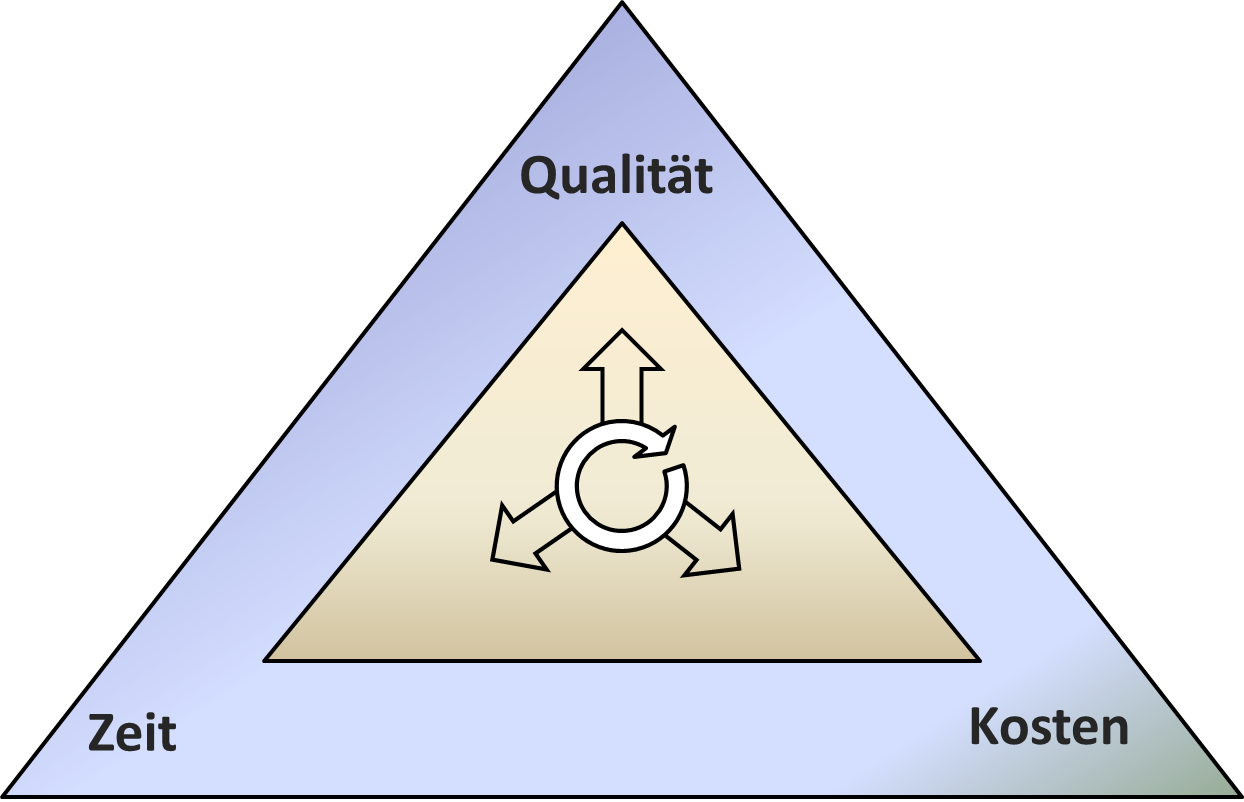
\includegraphics[width=1.1\textwidth]{../images/software_quality_triangle.PNG}
\caption[Software-Qualitätspyramide]{Software-Qualitätspyramide}
\label{fig:software_quality_triangle}
\end{figure}

Beispiel für eine Tabelle

\begin{table}[H]
\centering
\begin{tabular}{|l|p{9cm}|}
\hline
\rowcolor[HTML]{EFEFEF} 
\textit{\textbf{Qualitätsmerkmal}} & \textit{\textbf{Erläuterung}}       \\ \hline
\textbf{Änderbarkeit}              & Aufwand, der zur Durchführung vorgegebener Änderungen notwendig ist. Dies beinhaltet die Unterkategorien Änderungen, Analysierbarkeit, Modifizierbarkeit, Stabilität und Prüfbarkeit.
\\ \hline
\textbf{Benutzbarkeit}             &                                                                                                                                                                                                 Aufwand, den ein Benutzer der Software für das Verstehen und die Verwendung der Software aufbringen muss. Dieser beinhaltet die Unterkategorien Verständlichkeit, Erlernbarkeit und Bedienbarkeit.
 \\ \hline
\textbf{Effizienz}                 &                                                                                                                                                                                                    
Misst die Leistung der Software anhand des Zeitbedarfes, bei dessen Ausführen oder deren Ressourcenverbrauch.
\\ \hline
\textbf{Zuverlässigkeit}           &                                                                                                                                                                                                    
Eigenschaften, die ausdrücken, wie fehlertolerant eine Software ist, also wie intelligent auf Fehler reagiert wird.
\\ \hline
\textbf{Funktionalität}            &                                                                                                                                                                                                    
Die Übereinstimmung der Software mit der Spezifikation. Sie ist eine der wichtigsten Qualitätsmerkmale von Software, das ist die grundlegenden Eigenschaften zu den Funktionen der Software, was sie funktional leisten soll und wie. Darunter fallen, Richtigkeit, Angemessenheit, Ordnungsmäßigkeit, Interoperabilität und Sicherheit.
\\ \hline
\textbf{Übertragbarkeit}           &                                                                                                                                                                                                    
Sagt aus, ob eine Software auf unterschiedlichen Betriebssystemen mit verschiedener Hardwareausstattung ausgeführt werden kann.
\\ \hline
\end{tabular}
\caption{Qualitätsmerkmale und ihre Bedeutung für das Software-Produkt}
\label{quality_of_sortware}
\end{table}
Beispiel für eine Box mit Text

\fbox{\parbox{\columnwidth}{
Als Käufer möchte ich einen Artikel in meinen Warenkorb legen, damit ich diesen anschließend kaufen kann.
}}
 % fundamentals
\section{Bestehende Lösungen}
\label{sec:existing_solution} % existing solutions
\section{Konzept}
 Beispiel für ein Listing
\lstset{language=XML}
\begin{lstlisting}[caption={XML Definitionen},captionpos=b]
<?xml version="1.0" encoding="UTF-8"?>
<bpmn:definitions xmlns:bpmn="http://www.omg.org/spec/BPMN/20100524/MODEL" xmlns:bpmndi="http://www.omg.org/spec/BPMN/20100524/DI" xmlns:di="http://www.omg.org/spec/DD/20100524/DI" xmlns:dc="http://www.omg.org/spec/DD/20100524/DC" xmlns:xsi="http://www.w3.org/2001/XMLSchema-instance" id="Definitions_1" targetNamespace="http://bpmn.io/schema/bpmn" exporter="Camunda Modeler" exporterVersion="1.11.3">
</bpmn:definitions>
\end{lstlisting}
\label{sec:konzept} % concept
\section{Prototypische Implementierung}
\label{sec:prototyp}

\subsection{Anforderungsanalyse}

\subsubsection{Funktionale Anforderungen}

\subsubsection{Nicht-Funktionale Anforderungen} % prototype
\section{Evaluation}

\subsection{Zielsetzung}

\subsection{Konzept}

\subsection{Prototyp}

\subsection{Fazit} % evaluation
\section{Zusammenfassung und Ausblick}
\subsection{Zusammenfassung}

\subsection{Ausblick}
\label{sec:extension}
 % conclusion
\listoftables % add list of tables
\clearpage{}
\listoffigures % add list of figures 
\clearpage{}
\lstlistoflistings
\clearpage{}
\iftoggle{german}{
\def\AbbrvName{Abkürzungsverzeichnis}
}{
\def\AbbrvName{List of Abbreviations}
}
\section*{\AbbrvName}
\addcontentsline{toc}{section}{\AbbrvName}
\sectionmark{\AbbrvName}

\def\LongestAcro{wmSDN}
\begin{acronym}[\LongestAcro] % Pass the longest acronym here to align them correctly
\setlength{\itemsep}{-\parsep} % reduce the space between acronyms
 \acro{TA}{Test Automation}
 \acro{OS}{Operating System - Betriebssystem}
 \acro{BPMN}{Business Process Model and Notation - Eine grafische Spezifikationssprache in der Wirtschaftsinformatik und im Prozessmanagement}
 \acro{ISTQB}{International Software Testing Qualifications Board (http://www.istqb.org/)}
 \acro{XML}{„Extensible Markup Language“ - erweiterbare Auszeichnungssprache zur Darstellung hierarchisch strukturierter Daten in Form von Text}
 \acro{AE}{Automation Engine - Bestandteil der CA Automic Workload Automation }
 \acro{AWA}{CA Automic Workload Automation}
 \acro{VARA}{Variablen-Objekt der AWA, welches einen Schlüsselwert mit fünf dazugehörigen Werten speichert}
  \acro{b4A}{Kurzform für die Software b4Automic Solution}
 \acro{JOB}{Ausführbares-Objekt der AWA, was benutzt wird um z.B. OS Operationen auszuführen}
 \acro{USER}{Benutzer-Objekt der AWA}
\end{acronym}

 % include the acronym thing
\clearpage{}
% choose your type of citation here
%\bibliographystyle{plainnat} % author and year
%\bibliographystyle{amsalpha} % author and year short
\bibliographystyle{alphaabbr} % author short and year
%\bibliographystyle{alpha} % author and year
%\bibliographystyle{plain} % only numbers
%\bibliographystyle{unibonn_ay} % a special file used for the uni bonn
\singlespacing % bibliography with single spacing
% \nocite{*} % print all references in bib file regardless of citing
\bibliography{references}
\addcontentsline{toc}{section}{Literaturverzeichnis}
% Start of the appendix
\appendix 
% The appendix is a chapter
\iftoggle{german}{
\section{Anhang}
\label{sec:anhang}
%Hier muss alles rein!

}{
\section{Appendix}
}
\end{document}
